\section{Experiments}
\label{sec:eval}

%In this section, we evaluate the effectiveness and efficiency of
%our approach in computing the semantic similarity between terms.
In this section, we first outline the experimental setup,
and then compare the effectiveness of the online and the offline
variant of our approach, and also compare our approaches
(basic, refined and refined with pruning) with 12 competing
methods on three benchmark data sets.
Finally, we evaluate the efficiency of our approaches.
% in the context of other peers.

\subsection{Experiment Setup}
We use three data sets in the following experiments, including two well-known benchmark data sets for word similarity and one labeled data set
for evaluating MWEs which is created by us. Table~\ref{tab:dataSets} shows the descriptions and some examples in each of the three data sets.
M\&C data set is a subset of Rubenstein-Goodenough's \cite{Rubenstein:1965}
and consists of 28 word pairs.
Because of the omission of two word
pairs in earlier versions of WordNet, most researchers used only
28 word pairs for evaluations in the past. We follow this tradition in this paper.
WordSim203 is a subset from WordSim353\cite{wordSim:353}, and has been
used as a similarity testing data set by Agirre et. al.\cite{Agirre:2009}
It contains 203 pairs which are considered more similar than related.
%, where similar pairs include those
%classified as synonyms, antonyms, identical, or hyponym-hypernym, and unrelated pairs indicate those classified as none-of-the-above that had
%average similarity less than or equal to 0.5 (on a scale of 0 to 1).
Because there are no benchmark data for the semantic similarity between
MWEs, we labeled 300 pairs (known as WP) with both words and MWEs. Our labeled data consist of three categories: 100 concept-entity pairs, 100
concept-concept pairs and 100 entity-entity pairs. These 300 pairs contain 84 word pairs and 216 MWE pairs, in which 71 MWE pairs are in WordNet
the remaining are not. You can find all 300 labeled pairs at \url{http://adapt.seiee.sjtu.edu.cn/similarity/SimCompleteResults.pdf}.
%and the composition of word/MWE pairs is listed
%in Table~\ref{tab:pairDistribution}.
Five native speakers of English labeled these pairs according to the label classes, and the labels are then translated into numerical similarity
scores in Table~\ref{tab:manualLabels}. These scores are averaged to produce
the final rating for each pair.

All experiments are performed on
an Intel Core 2 Duo 2.66GHz PC with 4G physical memory,
running Windows 7 Enterprise. All timing results are averaged over 10 runs.
All competing methods involved in this section are summarized
in Table~\ref{tab:allmethods}. We implemented S\'{a}n method while adopting the existing implementation \cite{wordNetSim} of other methods.
%open source code at authors' homepage or they are encapsulated in an open source tool for WordNet-based similarity\cite{wordNetSim}.
To evaluate the effectiveness of each method,
we compute the Pearson Correlation Coefficient (PCC in short)
to measure the agreement between the machine rating
(computed by the semantic similarity measurement approaches) and
the human ratings over the data sets
as follows, where
$X$ is the machine ratings while $Y$ is the human ratings:
\begin{eqnarray*}\label{eq:PCC}
 \rho = \frac{\sum_{i=1}^n(X_i-\bar{X})(Y_i-\bar{Y})}{\sqrt{\sum_{i=1}^n(X_i-\bar{X})^2}\sqrt{\sum_{i=1}^n(Y_i-\bar{Y})^2}}
\end{eqnarray*}
%\KZ{Include the definition here.}\LP{added}

\begin{table}[th]
\centering
\caption{Data Sets Used in Experiments}
\label{tab:dataSets}
\small
\begin{tabular}{|c|c|c|}\hline
 M\&C   &WordSim203 similarity &Our labeled data\\
 data set\cite{Miller:1998} &\cite{Agirre:2009}(WS in short) &(WP in short)\\\hline\hline
 \multicolumn{3}{|l|}{~~~~~~~~~~~~~~~~~~~~~~~~~~~~~~~~~~\textbf{Type}}\\\hline
 Words & Words & Words \& MWEs \\\hline
 \multicolumn{3}{|l|}{~~~~~~~~~~~~~~~~~~~~~~~~~~~~~~~~~\textbf{\#Pairs}}\\\hline
  28 & 203 & 300 \\\hline
  \multicolumn{3}{|l|}{~~~~~~~~~~~~~~~~~~~~~~~~~~~~~~~\textbf{Examples}}\\\hline
 \pair{lobster}{food} &\pair{lobster}{wine}&\pair{animal}{poodle}\\\hline
\pair{chord}{smile} &\pair{professor}{doctor}&\pair{microsoft}{apple}\\\hline
&&$\langle$\emph{shell},~\emph{exxon}\\
\pair{bird}{cock} &\pair{tiger}{jaguar}&\emph{mobil~corp.}$\rangle$\\\hline
$\langle$\emph{crane},  &   &$\langle$\emph{caged~animal},\\
\emph{implement}$\rangle$   &$\langle$\emph{precedent},\emph{information}$\rangle$   &\emph{game~animal}$\rangle$\\\hline
\end{tabular}
\end{table}

%\begin{table}[th]
%\centering
%\caption{Experimental Data}
%\label{tab:dataSets}
%\scriptsize{
%\begin{tabular}{|c|c|c|c|}\hline
% &     &WordSim353  &\\
%  & M\&C   &similarity\cite{wordSim:353} &Our labeled data\\
% & database\cite{Miller:1998}  &(WS for short) &(WP for short)\\\hline\hline
%Type & Words & Words & Words \& MWEs \\\hline
%\#Pairs & 28 & 203 & 300 \\\hline
% &\pair{lobster}{food} &\pair{cup}{artifact}&\pair{animal}{poodle}\\\cline{2-4}
%&\pair{chord}{smile}   &\pair{doctor}{nurse}&\pair{microsoft}{apple}\\\cline{2-4}
%&&&$<$\emph{shell},~\emph{exxon}\\
%Examples&\pair{coast}{forest} &\pair{football}{tennis}&\emph{mobil~corp.}$>$\\\cline{2-4}
%&$<$\emph{crane},  &$<$\emph{deployment},  &$<$\emph{caged~animal},\\
%&\emph{implement}$>$   &\emph{departure}$>$    &\emph{game~animal}$>$\\\hline
%\end{tabular}
%}
%\end{table}

%\begin{table}[!t]
%\centering
%\caption{Experimental Data}
%\label{tab:dataSets}
%\small{
%\begin{tabular}{|c|c|c|c|}\hline
%Data source & type &\#pairs &Description\\\hline
%&  & & Judged by 51 human subjects\\
%database & word &28 & in a scale of [0.0, 4.0]\\\hline
%&  & & An average of 13-16 human\\
%(WS for short)\cite{wordSim:353} & word &203 &judgements in a scale of [0.0, 10.0]\\\hline
%& word and multi- & &An average of 5 human\\
%(WP for short)& word expression & 300& judgements in a scale of [0.0, 1.0]\\\hline
%\end{tabular}
%}
%\end{table}
%\begin{table}[!t]
%\centering
%\caption{Some Examples from Three databases}
%\label{tab:samplesOfDatasets}
%\small{
%\begin{tabular}{|c|c|c|}\hline
%M\&C database & WordSim353 similarity  &WP database\\\hline
%\pair{lobster}{food}   &\pair{cup}{artifact}   &\pair{microsoft}{apple}\\
%\pair{coast}{forest}   &\pair{deployment}{departure}   &\pair{marine animal}{cold-blooded animal}\\
%\pair{crane}{implement}    &\pair{doctor}{nurse}   &\pair{animal}{poodle}\\
%\pair{chord}{smile}    &\pair{football}{tennis}    &\pair{shell}{exxon mobil corp.}\\\hline
%\end{tabular}
%}
%\end{table}

%\begin{table}[th]
%\centering
%\caption{Distributions of Pairs in WP}
%\label{tab:pairDistribution}
%\small{
%\begin{tabular}{|c|c|c|c|}\hline
%&Word & MWE & Total\\\hline\hline
%\#Pairs &84 & 216 & 300\\
%\#Identified by WordNet & 75 & 71&146\\\hline
%\end{tabular}
%}
%\end{table}

\begin{table}[th]
\centering
\caption{Label Classes and Similarity Scores}
\label{tab:manualLabels}
\small{
\begin{tabular}{|c|c|}\hline
Label Classes   & Similarity Score\\\hline\hline
Very similar    &1\\
Fairly similar  &0.75\\
Don't know  &0.5\\
Fairly different    &0.25\\
Very different  &0\\\hline
\end{tabular}
}
\end{table}

\begin{table}[th]
\centering
\caption{Competing Methods (IC = Information Content, LCA = Least Common Ancestor)}
\label{tab:allmethods}
\small
\begin{tabular}{|l|l|}\hline
{\bf Approach} & {\bf Description} \\\hline\hline
Hungarian (Hun) \cite{hungarian:string}     &string-based\\\hline
Tray (Tra)\cite{tray:2005} &string-based+WordNet \\ \hline
Rada (Rad) \cite{Rada:1989} &path-based (WordNet) \\\hline
Hirst (Hir) \cite{Hirst:1998}   &lexical chain-based (WordNet) \\\hline
Do \cite{Do:DRSTV09}    &lexical chain-based (WordNet) \\\hline
Resnik (Res)\cite{Resnik:1995}  & IC of LCA $+$WordNet \\\hline
Jcn \cite{Jiang:1997}   & IC of LCA + the term + WordNet \\\hline
Lin \cite{Lin:1998} & IC of LCA + the term + WordNet\\\hline
S\'{a}nchez (S\'{a}n)\cite{Snchez:2011} & IC of leaves and parents + WordNet \\\hline
Banerjee (Ban)\cite{Banerjee:2002}  & glosses-based (WordNet) \\\hline
Agirre (Agi)\cite{Agirre:2010}  & personalized PageRank (WordNet)\\\hline
Bollegala (Bol)\cite{Bollegala:2011} &search-snippet-based  \\\hline
Basic & Our basic approach\\\hline
RC & Our refined approach \\\hline
RCP & Our refined approach with pruning \\\hline
\end{tabular}
\end{table}

%\begin{table*}[th]
%\centering
%\caption{Pearson Correlation Coefficient on Three Data Sets
%with Word or MWE pairs}
%\label{tab:benchmarkData}
%\small{
%\begin{tabular}{|c|c|c|c|c|c|c|c|}\hline
%%  &   \multicolumn{3}{c|}{} &\multicolumn{2}{c|}{Pairs with multi-}\\
%&  \multicolumn{4}{c|}{Word Pairs} &\multicolumn{3}{c|}{MWE Pairs}\\\hline
%   &   & &75 pairs & total 278 pairs &71 pairs & 145 pairs &total 216 pairs \\ %&146 pairs\\
%Method &M\&C &WS & in WordNet & &in WordNet &not in WordNet &  \\ \hline\hline % & in WP\\\hline\hline
%Hun    &-0.196 &0.064 &0.039&0.049 &0.371 &0.429&0.355\\ \hline % &0.093\\\hline
%Tra    &0.755  &0.594 &0.520&0.579 &0.389 &0.325&0.344\\ \hline %&0.459\\\hline
%Rad&0.739  &0.595&0.520&0.569&0.592    &-&-\\ \hline %&0.557\\\hline
%Hir    &0.643  &0.574&0.533&0.552&0.459    &-&-\\ \hline %&0.504\\\hline
%Do &0.676  &0.482&0.355&0.440&0.359    &-&-\\ \hline %&0.344\\\hline
%Res&0.762  &0.672&0.573&0.643&0.744    &-&-\\ \hline %&0.677\\\hline
%Jcn&0.848  &0.371&0.641&0.285&0.382    &-&-\\ \hline %&0.432\\\hline
%Lin&0.822  &0.674&0.605&0.658&0.717    &-&-\\ \hline %&0.678\\\hline
%San&0.865  &0.690  &0.675  &0.681&0.740    &-&-\\ \hline %&0.701\\\hline
%Ban&0.781  &0.651&0.470&0.594&0.377     &-&-\\ \hline %&0.428\\\hline
%Agi&0.795  &0.579&0.570&0.359&0.380     &-&-\\ \hline %&0.465\\\hline
%Bol&0.834  &0.564& 0.466&0.523&0.592 &0.511&0.498\\ \hline %& 0.478\\\hline
%Basic&0.777    &0.576 &0.321&0.446&0.313    &0.449&0.440\\ \hline %&0.356\\\hline
%RC &0.885  &0.690 &0.452&0.484&0.651    &0.635&0.595\\ \hline %&0.520\\\hline
%RCP&\textbf{0.921}&\textbf{0.725} &\textbf{0.772}&\textbf{0.767}&\textbf{0.822} &\textbf{0.665}&\textbf{0.670}\\ \hline %&\textbf{0.760}\\\hline
%\end{tabular}
%}
%\end{table*}
%\begin{table*}[th]
%\centering
%\caption{Pearson Correlation Coefficient on Three Data Sets
%with Word or MWE Pairs}
%\label{tab:benchmarkData}
%\small{
%\begin{tabular}{|c|c|c|c|c||c|c|c|}\hline
%%   &   \multicolumn{3}{c|}{} &\multicolumn{2}{c|}{Pairs with multi-}\\
%&   \multicolumn{4}{c||}{Word Pairs} &\multicolumn{3}{c|}{MWE Pairs}\\\hline
%    &   & & Words & & MWE Pairs & MWE Pairs & \\ %&146 pairs\\
%Method  &M\&C &WS & from WP & All Word Pairs &in WordNet &Not in WordNet & All MWE Pairs \\ \hline\hline % & in WP\\\hline\hline
%Hun &-0.196 &0.064 &0.015&0.038 &0.371 &0.429&0.355\\ \hline % &0.093\\\hline
%Tra &0.755  &0.594 &0.379&0.480 &0.389 &0.325&0.344\\ \hline %&0.459\\\hline
%Rad&0.739   &0.595&0.395&0.510&0.592    &-&-\\ \hline %&0.557\\\hline
%Hir &0.643  &0.574&0.451&0.511&0.459    &-&-\\ \hline %&0.504\\\hline
%Do  &0.676  &0.482&0.322&0.419&0.359    &-&-\\ \hline %&0.344\\\hline
%Res&0.762   &0.672&0.424&0.569&0.744    &-&-\\ \hline %&0.677\\\hline
%Jcn&0.848   &0.371&0.382&0.275&0.382    &-&-\\ \hline %&0.432\\\hline
%Lin&0.822   &0.674&0.446&0.579&0.717    &-&-\\ \hline %&0.678\\\hline
%S\'{a}n&0.865   &0.690  &0.643&0.655&0.740  &-&-\\ \hline %&0.701\\\hline
%Ban&0.781   &0.651&0.426&0.560&0.377     &-&-\\ \hline %&0.428\\\hline
%Agi&0.795   &0.579&0.258&0.343&0.380     &-&-\\ \hline %&0.465\\\hline
%Bol&0.834   &0.564& 0.476&0.523&0.592 &0.511&0.498\\ \hline %& 0.478\\\hline
%Basic&0.777 &0.576 &0.387&0.429&0.313    &0.449&0.440\\ \hline %&0.356\\\hline
%RC  &0.885  &0.690 &0.457&0.494&0.651    &0.635&0.595\\ \hline %&0.520\\\hline
%RCP&\textbf{0.921}&\textbf{0.725} &\textbf{0.811}&\textbf{0.770}&\textbf{0.822} &\textbf{0.665}&\textbf{0.670}\\ \hline %&\textbf{0.760}\\\hline
%\end{tabular}
%}
%\end{table*}

\begin{table}[th]
\centering \caption{Pearson Correlation Coefficient on Three Data Sets with Word or MWE Pairs (WN: WordNet)} \label{tab:benchmarkData}
\scriptsize{
\begin{tabular}{|p{23pt}|p{18pt}|p{15pt}|p{19pt}|p{16pt}||p{21pt}|p{23pt}|p{17pt}|}\hline
%   &   \multicolumn{3}{c|}{} &\multicolumn{2}{c|}{Pairs with multi-}\\
&   \multicolumn{4}{c||}{Word Pairs} &\multicolumn{3}{c|}{MWE Pairs}\\\hline
    &   & & Words &~All& MWEs &  MWEs &~All\\ %&146 pairs\\
Method  &M\&C &WS &~from  &  Word  &~~~in  &Not in  &  MWE \\
  && &~WP &  Pairs &~~WN & ~~WN & Pairs \\
\hline\hline % & in WP\\\hline\hline
Hun &-0.20 &0.06 &0.02&0.04 &0.37 &0.43&0.36\\ \hline % &0.093\\\hline
Tra &0.76  &0.59 &0.38&0.48 &0.39 &0.33&0.34\\ \hline %&0.459\\\hline
Rad&0.74   &0.60&0.40&0.51&0.59    &-&-\\ \hline %&0.557\\\hline
Hir &0.64  &0.57&0.45&0.51&0.46    &-&-\\ \hline %&0.504\\\hline
Do  &0.68  &0.48&0.32&0.42&0.36    &-&-\\ \hline %&0.344\\\hline
Res&0.76   &0.67&0.42&0.57&0.74    &-&-\\ \hline %&0.677\\\hline
Jcn&0.85   &0.37&0.38&0.28&0.38    &-&-\\ \hline %&0.432\\\hline
Lin&0.82   &0.67&0.45&0.58&0.72    &-&-\\ \hline %&0.678\\\hline
S\'{a}n&0.87   &0.69  &0.64&0.66&0.74  &-&-\\ \hline %&0.701\\\hline
Ban&0.78   &0.65&0.43&0.56&0.38     &-&-\\ \hline %&0.428\\\hline
Agi&0.80   &0.58&0.26&0.34&0.38     &-&-\\ \hline %&0.465\\\hline
Bol&0.83   &0.56& 0.48&0.52&0.59 &0.51&0.50\\ \hline %& 0.478\\\hline
Basic&0.78 &0.58 &0.39&0.43&0.31    &0.45&0.44\\ \hline %&0.356\\\hline
RC  &0.89  &0.69 &0.46&0.49&0.65    &0.64&0.60\\ \hline %&0.520\\\hline
RCP&\textbf{0.92}&\textbf{0.73} &\textbf{0.81}&\textbf{0.77}&\textbf{0.82} &\textbf{0.67}&\textbf{0.67}\\ \hline %&\textbf{0.760}\\\hline
\end{tabular}
}
\end{table}

%\begin{table*}[!t]
%\centering
%\caption{Pearson correlation coefficient on 146 labeled data identified by WordNet}
%\label{tab:146pairs}
%\begin{tabular}{|l|l|c|c|c|}\hline
%~~~~~~~~~Approach  &~~~~~~~~~~~~~~~Source  &on 75 pairs    &on 71 pairs    &on 146 pairs\\\hline
%Hungarian method   &string-based   &0.0391 &0.3712&    0.0931\\\hline
%Tray's (2005)  &string-based+WordNet   &0.5201 &0.3887 &0.4594\\\hline
%Rada's (1989)  &path-length-based (WordNet)    &0.5195 &0.5915 &0.5568\\\hline
%Hirst's (1998) &lexical chain-based  (WordNet) &0.5334 &0.4586 &0.5036\\\hline
%Do's (2009)    &lexical chain-based (WordNet)  &0.3550 &0.3586 &0.3438\\\hline
%resnik's (1995)    &information content+WordNet    &0.5727 &0.7438 &0.6773\\\hline
%jcn's (1997)   &information content+WordNet    &0.6408 &0.3819 &0.4319\\\hline
%lin's (1998)   &information content+WordNet    &0.6048 &0.7169 &0.6777\\\hline
%Banerjee's (2002)  &glosses-based (WordNet)    &0.4698 &0.3768 &0.4279\\\hline
%Eneko's (2010) &personalized PageRank (WordNet)    &0.5696 &0.3802 &0.4650\\\hline
%our basic approach &semantic network-based &0.3212 &0.3125 &0.3557\\\hline
%clustering-based &semantic network+clustering  &0.4521 &0.6506 &0.5195\\\hline
%our clustering approach    &semantic network+clustering+clusterPrunning    &\textbf{0.7716}     &\textbf{0.8215}   &\textbf{0.7601}\\\hline
%\end{tabular}
%\end{table*}

%\begin{table*}[!t]
%\centering
%\caption{Pearson correlation coefficient on pairs with multi-word expression from WP identified by WordNet}
%\label{tab:146pairs}
%\begin{tabular}{|l|l|c|c|}\hline
%~~~~~~~~~Algorithm &~~~~~~~~~~~~~~~Technique   &71 pairs from WP &146 pairs from WP\\\hline
%Hungarian method   &string-based       &0.3712&    0.0931\\\hline
%Tray's (2005)  &string-based+WordNet       &0.3887 &0.4594\\\hline
%Rada's (1989)  &path-length-based (WordNet)    &0.5915 &0.5568\\\hline
%Hirst's (1998) &lexical chain-based  (WordNet)     &0.4586 &0.5036\\\hline
%Do's (2009)    &lexical chain-based (WordNet)      &0.3586 &0.3438\\\hline
%Resnik's (1995)    &information content+WordNet        &0.7438 &0.6773\\\hline
%Jcn's (1997)   &information content+WordNet        &0.3819 &0.4319\\\hline
%Lin's (1998)   &information content+WordNet        &0.7169 &0.6777\\\hline
%Banerjee's (2002)  &glosses-based (WordNet)        &0.3768 &0.4279\\\hline
%Agirre's (2010)    &personalized PageRank (WordNet)        &0.3802 &0.4650\\\hline
%Bollegala's (2011)\cite{Bollegala:2011}*   &search-snippet-based   &0.5916& 0.4781\\\hline
%our basic approach &semantic network-based     &0.3125 &0.3557\\\hline
%clustering-based &semantic network+clustering      &0.6506 &0.5195\\\hline
%clustering-based+clusterPruning    &semantic network+clustering    &\textbf{0.8215}     &\textbf{0.7601}\\\hline
%\end{tabular}
%\end{table*}

\subsection{Effectiveness}
Figure~\ref{fig:online-offiline} reports the PCC in our RCP
approach with online clustering and offline
clustering respectively on the WP data set.
From this figure, we can see that the PCC values for
online clustering and offline clustering differ only marginally.
%approach with online clustering is only improved by 0.01
%at most compared to that with offline clustering.
%This indicates our RCP approach with offline clustering is
%comparable to that with online clustering.
Therefore, in the following experiments,
we use the offline clustering in our refined approach.

Table~\ref{tab:benchmarkData} compares the PCC of our approaches with that of 12 others. Some of these competing methods (from Rad to Agi) rely
on WordNet and do not recognize MWEs that are not in WordNet, therefore they are excluded from comparison in the experiment on ``MWEs Not in
WordNet'', marked with ``-''.
%Because not every one of the 12 methods
%works with arbitrary MWEs, the data sets used in this experiment include
%only words and those MWEs that are included in WordNet, to have a fair
%comparison. In particular 2 subsets of WP are used, namely the 75 pairs of
%words and 71 pairs of MWEs indentified by WordNet.
From the experimental results, we make the following observations.

First, our most advanced approach, RCP, leads the competition
against the peers by large margins in all data sets,
especially in MWE pairs.
%\item Compared to the string-based methods such as Hun and Tra,
%the RCP approach can improve the PCC value by more than 0.17.

Second, in the Hun method, the PCC value is negative,
because it depends only on the
surface forms of terms. Most terms which are
semantically similar are not lexically similar.
Thus, some of the computed similarities are incorrect , which leads
to the negative correlation.

Third, methods based on taxonomy structure, such as Rad, Hir and Do,
generally fare better than pure syntax-based methods.
%\item Considering the ontology structure considering methods such as
%Rad, Hir and Do, we find the Rad method using the minimum path-length in WordNet outperforms other methods using lexical chains. Compared to the best result in these methods, our RCP approach can improve the PCC value by the range of [0.11, 0.41].

Fourth, information content based methods, such as
Res, Jcn, Lin and S\'{a}n, generally do better than other WordNet based
methods.
%, and narrow the gap with our approaches but RCP is still
%approximately 0.1 ahead.
Information content based methods
effectively combines the knowledge from the taxonomy structure
and external corpora. This has certain advantage but the coverage of
this knowledge is still limited compared to the knowledge we acquired
from the entire web.
%the advantage of our RCP approach is reduced, the PCC value is improved by 0.09 at most. This is because these methods consider the information contexts of terms in the calculation of the semantic similarity between terms besides considering the ontology structures of terms in WordNet, which improves the accuracy of similarity measurement compared to Rad, Hir and Do.
%\item Considering other WordNet-based methods such as Ban and Agi,
%the Ban method introduces the glosses to improve the accuracy of
%similarity measurement especially for ambiguous terms while Agi
%uses the random-walk model to get the probability of each term in WordNet,
%but their PCC values are still lower than our RCP approach by the range of [0.07, 0.28].

Finally, search snippet-based method like Bol works fine with M\&C data sets but fares quite badly elsewhere. This is because it considers
co-occurrences of two terms which produces more of relatedness than similarity.  It works badly with words in WP because word pairs in WP
contain many ambiguous terms, and many pairs with transitive isA relationships ( e.g., \pair{animal}{puppy} with ``dog'' being the child of
``animal'' and parent of ``puppy'') and many pairs with vague senses (e.g., \pair{music}{lunch} with the vague sense ``activity'').
Co-occurrence alone is not effective on these pairs.
%our RCP approach can improve the PCC value by the range of [0.08, 0.30]. This is because the Bol method first considers the co-occurrences of two terms, which probably lead to get higher similarity for those relevant terms.
%\item Compared to our Basic approach, RC can improve the PCC value by 0.11
%at least and RCP can further improve the PCC value by the range of [0.04, 0.32].
%These data reveals that the RCP approach outperforms all of
%the state-of-the art semantic similarity calculation methods mentioned
%above as well as our Basic and RC approaches.
%\KZ{It's NOT database, but data set. Change everywhere including
%graphs.}

Figure~\ref{fig:ComparisonOn300pairsAllMethods} reports
the PCC of six approaches which work with arbitrary MWEs and the
experiment is done on all 300 pairs from the WP data set.
%We can observe the following these results.
RCP produces a PCC value of around 0.7 which is much higher
than the other peers.
%Our Basic approach improves the PCC value by 0.15 at most compared
%to the string-based methods of Hun and Tra while it is lower than
%the Bol method by 0.06. However, RC and RCP approaches significantly
%improve the PCC value by 0.16 and 0.24 respectively compared to
%the best one score by the other four approaches.

Figure~\ref{fig:Pearson-Performance-on-different-types-of-pairs} reports the PCC of our approaches on three types of pairs in WP. From the
experimental results, we can see that our three approaches have the same PCC value (0.74) on the concept pairs, because they have the same
calculation mechanism on these pairs. Our methods generally work better with concept-entity pairs than entity-entity pairs. The reason is that
concept-entity pairs are similar only if they are in a hypernym-hyponym relation so the similarity is clearly defined. In the case of
entity-entity pairs, comparing their concept contexts can be difficult due to i) the ambiguity in the senses and ii) the noises in the
super-concepts
which can be very abstract and vague. %\KZ{Is the above reasoning
%correct?}

Table~\ref{tab:exampleOfOurResults} shows some examples from each data set along with the computed similarity scores by the RCP approach. Human
ratings have been uniformly normalized to [0, 1] in this table. Complete set of results can be found at
\url{http://adapt.seiee.sjtu.edu.cn/similarity/}.
%However, on the entity pairs and concept-entity pairs,
%RCP has clear advantage over the other two methods.
%RCP results are on average 0.46 higher than the Basic method on entity pairs,
%and 0.23 higher on concept-entity pairs. These data show that our clustering-based approach
%with cluster pruning can largely improve the accuracy of computing the semantic similarity between terms compared to our Basic and RC approaches.

%\begin{figure*}[th]
% \centering
%\begin{minipage}[b]{0.32\textwidth}
% \includegraphics[width=\textwidth]{performanceCompareInOnlineAndOffline.eps}
% \caption{Performance of RCP with online/offline clustering}
% \label{fig:online-offiline}
%\end{minipage}
%\hfill
%\begin{minipage}[b]{0.32\textwidth}
% \includegraphics[width=\textwidth]{ComparisonOn300pairsAllMethods.eps}
% \caption{Performance comparison on WP}
% \label{fig:ComparisonOn300pairsAllMethods}
%\end{minipage}
%\hfill
%\begin{minipage}[b]{0.32\textwidth}
% \includegraphics[width=\textwidth]{Pearson-Performance-on-different-types-of-pairs.eps}
% \caption{Performance comparison on various types of pairs}
% \label{fig:Pearson-Performance-on-different-types-of-pairs}
%\end{minipage}
%\end{figure*}

\begin{figure}[!t]
 \centerline{
 \includegraphics[width=0.98\columnwidth]{performanceCompareInOnlineAndOffline.eps}}
 \caption{Performance of RCP with online/offline clustering}
 \label{fig:online-offiline}
\end{figure}

\begin{figure}[!t]
 \centerline{
  \includegraphics[width=0.98\columnwidth]{ComparisonOn300pairsAllMethods.eps}}
 \caption{Performance comparison on WP}
 \label{fig:ComparisonOn300pairsAllMethods}
\end{figure}

\begin{figure}[!t]
 \centerline{
  \includegraphics[width=0.98\columnwidth]{Pearson-Performance-on-different-types-of-pairs.eps}}
 \caption{Performance comparison on various types of pairs}
 \label{fig:Pearson-Performance-on-different-types-of-pairs}
\end{figure}

%\begin{figure*}[th]
%\begin{minipage}[bh]{0.32\textwidth}
% \centering
% \includegraphics[width=\textwidth]{performanceCompareInOnlineAndOffline.eps}
% \caption{Performance of RCP with online/offline clustering}
% \label{fig:online-offiline}
%\end{minipage}
%%\hfill
%\hspace{2pt}
%\begin{minipage}[bh]{0.32\textwidth}
% \centering
% \includegraphics[width=\textwidth]{ComparisonOn300pairsAllMethods.eps}
% \caption{Performance comparison on WP}
% \label{fig:ComparisonOn300pairsAllMethods}
%\end{minipage}
%%\hfill
%\hspace{2pt}
%\begin{minipage}[bh]{0.32\textwidth}
% \centering
% \includegraphics[width=\textwidth]{Pearson-Performance-on-different-types-of-pairs.eps}
% \caption{Performance comparison on various types of pairs}
% \label{fig:Pearson-Performance-on-different-types-of-pairs}
%\end{minipage}
%\end{figure*}

\begin{figure}[th]
 \centerline{
 \includegraphics[width=0.5\textwidth]{TimeComparisonOfOfflineAndOnline.eps}}
 \caption{Execution time in online/offline clustering}
 \label{fig:TimeComparisonOfOfflineAndOnline}
\end{figure}

\begin{figure}[th]
 \centerline{
 \includegraphics[width=0.5\textwidth]{TimecomparisonOfDiffApproaches.eps}}
 \caption{Computation time in different approaches}
 \label{fig:TimecomparisonOfDiffApproaches}
\end{figure}

\begin{figure}[th]
 \centerline{
 \includegraphics[width=0.5\textwidth]{Time-Performance-on-different-types-of-pairs.eps}}
 \caption{Computation time on different types of pairs}
 \label{fig:Time-Performance-on-different-types-of-pairs}
\end{figure}


%\begin{figure*}[th]
%\begin{minipage}[bh]{0.32\textwidth}
% \centering
% \includegraphics[width=\textwidth]{TimeComparisonOfOfflineAndOnline.eps}
% \caption{Execution time in online/offline clustering}
% \label{fig:TimeComparisonOfOfflineAndOnline}
%\end{minipage}
%\hspace{2pt}
%\begin{minipage}[bh]{0.32\textwidth}
% \centering
% \includegraphics[width=\textwidth]{TimecomparisonOfDiffApproaches.eps}
% \caption{Computation time in different approaches}
% \label{fig:TimecomparisonOfDiffApproaches}
%\end{minipage}
%\hspace{2pt}
%\begin{minipage}[bh]{0.32\textwidth}
% \centering
% \includegraphics[width=\textwidth]{Time-Performance-on-different-types-of-pairs.eps}
% \caption{Computation time on different types of pairs}
% \label{fig:Time-Performance-on-different-types-of-pairs}
%\end{minipage}
%\end{figure*}

%\begin{figure}[t]
% \centerline{
% \includegraphics[width=0.45\textwidth]{ComparisonOn300pairsAllMethods.eps}}
%\caption{Performance comparison on 300 pairs} \label{fig:ComparisonOn300pairsAllMethods}
%\end{figure}
%
%\begin{figure}[t]
% \centerline{
% \includegraphics[width=0.5\textwidth]{Pearson-Performance-on-different-types-of-pairs.eps}}
%\caption{Performance comparison on different types of pairs} \label{fig:Pearson-Performance-on-different-types-of-pairs}
%\end{figure}

%\begin{table}[th]
%\centering
%\caption{Examples of Computation Results in Our RCP approach}
%\label{tab:exampleOfOurResults}
%{
%\begin{tabular}{|l|c|}\hline
%pair & similarity score\\\hline
%\multicolumn{2}{|c|}{on M\&C data set}\\\hline
%\pair{bird}{cock} &    0.824\\\hline
%\pair{boy}{lad}    &0.800\\\hline
%\pair{coast}{shore}    &0.800\\\hline
%\pair{bird}{crane} &0.564\\\hline
%\pair{crane}{implement}    &0.294\\\hline
%\pair{monk}{oracle}    &0.002\\\hline
%\pair{journey}{car}    &0.001\\\hline
%\pair{lad}{wizard} &0.000\\\hline
%\multicolumn{2}{|c|}{on WS data set}   \\\hline
%\pair{tiger}{jaguar}   &0.979\\\hline
%\pair{professor}{doctor}   &0.930\\\hline
%\pair{vodka}{brandy}   &0.929\\\hline
%\pair{journey}{voyage} &0.800\\\hline
%\pair{travel}{activity}    &0.532\\\hline
%\pair{consumer}{energy}    &0.518\\\hline
%\pair{man}{governor}   &0.506\\\hline
%\pair{precedent}{information}  &0.011\\\hline
%\multicolumn{2}{|c|}{on WP data set}       \\\hline
%\pair{caged animal}{game animal}   &0.996\\\hline
%\pair{bank}{citibank}  &0.966\\\hline
%\pair{business}{restaurant}    &0.938\\\hline
%\pair{date}{asian pear}    &0.711\\\hline
%\pair{range}{food processor}   &0.689\\\hline
%\pair{climacteric fruit}{vegetable juice}  &0.226\\\hline
%\pair{apple}{garlic}   &0.019\\\hline
%\pair{music}{lunch}    &0.012\\\hline
%\end{tabular}
%}
%\end{table}

\begin{table}[th]
\centering \caption{Example Pairs and Their Semantic Similarity Scores Computed by RCP Approach
%{\color{red}(Human Ratings are
%normalized into [0,1] in this table)}
} \label{tab:exampleOfOurResults} {
\small
\begin{tabular}{|l|c|c|}\hline
&Human& Similarity\\
Pair &Rating& Score\\\hline \multicolumn{3}{|c|}{From M\&C Data Set}\\\hline \pair{furnace}{stove}   &0.778&0.950\\\hline \pair{bird}{cock}
&0.763&0.824\\\hline \pair{boy}{lad} &0.940&0.800\\\hline \pair{coast}{shore} &0.925&0.800\\\hline \pair{bird}{crane} &0.743 &0.564\\\hline
\pair{lobster}{food}&0.223 &0.525\\\hline \pair{crane}{implement}&0.420 &0.294\\\hline \pair{monk}{oracle}&0.275 &0.002\\\hline
\pair{journey}{car} &0.290&0.001\\\hline \pair{chord}{smile} &0.033&0.000\\\hline \multicolumn{3}{|c|}{From WS Data Set}  \\\hline
\pair{tiger}{jaguar} &0.800&0.979\\\hline \pair{professor}{doctor} &0.662&0.930\\\hline \pair{vodka}{brandy} &0.813 &0.929\\\hline
\pair{journey}{voyage} &0.929&0.800\\\hline \pair{travel}{activity} &0.500&0.532\\\hline \pair{consumer}{energy} &0.475&0.518\\\hline
\pair{man}{governor} &0.525&0.506\\\hline \pair{reason}{hypertension} &0.231&0.036\\\hline \pair{precedent}{information} &0.385  &0.011\\\hline
\pair{lobster}{wine} &0.570   & 0.000\\\hline
\multicolumn{3}{|c|}{From WP Data Set}
\\\hline \pair{caged~animal}{game~animal} &0.850&0.996\\\hline \pair{business}{restaurant} &0.550&0.938\\\hline \pair{shell}{exxon~mobil~corp.}
&0.850&0.814\\\hline \pair{animal}{poodle} &0.800  &0.720\\\hline \pair{date}{asian~pear} &0.500&0.711\\\hline \pair{range}{food~processor}
&0.750&0.689\\\hline \pair{climacteric~fruit}{vegetable~juice} &0.600  &0.226\\\hline \pair{music}{lunch} &0.100&0.012\\\hline
\pair{banana}{beef} &0.350&0.007\\\hline \pair{apple}{ipad}&0.200  &0.006\\\hline
\end{tabular}
}
\end{table}

\subsection{Efficiency}
Figure~\ref{fig:TimeComparisonOfOfflineAndOnline} compares the execution time between online clustering and offline clustering in our refined
approach. Offline clustering, with only a fraction of the cost, is a clear winner.
%Offline clustering clearly saves a lot of time in
%Figure~\ref{fig:TimeComparisonOfOfflineAndOnline}.
%compares the execution time between online clustering and offline clustering in our refined
%approach. Offline clustering, with only a fraction of the cost, is a clear winner.
%where the execution time of online clustering indicates the time cost of clustering the given concepts of the term, while the execution time of offline clustering indicates the time cost of finding clusters according to the clustering results in $\Gamma_{cluster}$. From the experimental results, we can see that the time complexity of online clustering is approximately in a direct proportion to the number of clustering objects (namely the count of concepts the given term belongs to), while the time complexity of offline clustering is almost a const value. More precisely, as the number of the concepts increases from 100 from 2000, the execution time of online clustering varies from 770 milliseconds to 2582 milliseconds while the execution time of offline clustering is always no more than 5 milliseconds. These data reveal that offline-clustering is more efficient, which is conducive to improve the efficiency in the calculation of the semantic similarity between terms.

Figure~\ref{fig:TimecomparisonOfDiffApproaches} reports the average computation time on a pair of terms in our approaches compared to the other
competitors. On average, RCP takes 65 milliseconds to compute the similarity of a pair, which is on par with most of the earlier methods using
information content and WordNet. String-based methods are faster for an obvious reason: they need not collect any context or model the context.
%Two methods are significantly slower than RCP and the crowd.
Hir is slow because it considers the lexical chain in the taxonomy in the
calculation of semantic similarity between terms.
%It requires traveling the
%taxonomy tree to find the hypernym and hyponym of terms. %\KZ{But why this slow??}
Bol takes about 60 times longer than RCP because
it requires extracting lexico-syntactic patterns from snippets online.
%which is very time consuming.
%It is slower than the string-based method of Hun and Tra.
%This is because the string-based methods needn't collecting any
%contexts of terms and modeling the contexts.
%However, as compared to the path-based and lexical chain-based methods,
%it is faster than the Hir and Do methods, which is less than
%1/2 of their time cost, while it is slower than the Rad method
%by 14 milliseconds.
%while Rad only use the minimum path length.
%The former especially the Hir method requires traveling the
%taxnomy tree to find the hypernym and hyponym information of terms.
%As compared to the IC-based methods, it is comparable to
%the Res, Jcn, Lin and San methods. For these IC-based methods,
%all IC values of terms involved in WordNet are prepared well, the only time consumption lies in the traveling of ontology tree. As compared to the glossed-based method Ban and the PageRank-based method Agi, it only consumes 1/2 of their time cost. This is because Ban needs to compare all glosses of the given term, and Agi needs to compute the probability of a random-walk initiated in the target word to reach any synset following the relations in WordNet.
%As compared to our Basic approach, because RCP needs clustering all concept contexts, which consumes more time. It is hence slower than Basic by 14 milliseconds. However, it is faster than RC by 100 milliseconds. This is because RC produces much more small sized clusters than RCP, and it needs comparing each pair of clusters to get the maximum one while RCP only maintains large sized clusters by cluster pruning. Though cluster pruning introduces the additional time consumption, it is much lower than the total time consumption in the comparing each pair of clusters in RC.

Figure \ref{fig:Time-Performance-on-different-types-of-pairs} shows
the average computation time on different types of pairs
using our approaches.
%From the experimental results, we observe the following.
%First, our three approaches can get the semantic similarity of a
%concept pair in 24 milliseconds.
%Second, on the entity pair and the concept-entity pair,
%RCP is comparable to Basic.
%Both approaches demand a lighter time overhead compared to RC.
%More specifically, Basic and RCP averagely consume 47 milliseconds
%and 125 milliseconds on an entity pair and a concept-entity pair
%respectively while RC consumes 216 milliseconds and 252 milliseconds
%respectively.
RCP costs less than half the time of RC due to the pruning.
%\KZ{Is this correct?}
Computing similarity between
concept-entity pairs is more expensive
because in order to catch the concept-entity pairs
with potentially transitive isA relationships, e.g., ``animal'' and
``puppy'' (with ``dog'' being the child of ``animal'' and parent
of ``puppy''), we iteratively check the relations between
every top ancestor concepts of an entity term and
the concept term in RCP. %\KZ{Check if the above is correct.}
%This imposes the computation time compared to that on
%the entity pair and concept pair.
%?gIn an overall considering,
%?gthe computation time on a pair is averagely 51 milliseconds,
%?g164 milliseconds and 66 milliseconds respectively in our
%?gBasic, RC and RCP approaches.

%\begin{table}[!h]
%\centering
%\caption{Case Study of Refined Approach}
%\label{tab:examples}{\scriptsize
%\begin{tabular}{|c|c|c|c|}\hline
% & &Basic & Refined \\
%termA & termB   & in Eq.~\ref{eq:cosine} & in Eq.~\ref{eq:clusterCosine}\\\hline
%\textbf{Apple} &Pear    &0.916  &\textbf{0.999}\\
%\textbf{Apple}&Microsoft        &\textbf{0.378} &\textbf{0.994}\\
%\textbf{Orange}&Pear    &0.715  &\textbf{0.845}\\
%\textbf{Orange}&Red     &\textbf{0.491} &\textbf{0.982}\\
%Microsoft&\textbf{GE}   &0.620  &\textbf{0.982}\\
%Music&Lunch     &0.012  &\textbf{0.884}\\
%Company&Microsoft       &0.930  &\textbf{0.934}\\
%Asia~country &Developing~country        &0.852  &0.852\\
%Country&Company &0      &0\\
%\hline
%\end{tabular}}
%\end{table}

%\begin{figure*}[t]
% \centerline{
% \includegraphics[width=0.9\textwidth]{Performance-on-different-types-of-pairs.eps}}
%\caption{Performance comparison in our approaches on different types of pairs} \label{fig:Performance-on-different-types-of-pairs}
%\end{figure*}
